% Source: printed p. 99; PDF p. 108
\noindent\textbf{Bài tập 3.4.4.6.} Cho $X$ là phức đơn hình sau, nên $X_0=\{A,B,\ldots,M\}$.
% Source diagram: Art_P78.jpg, visually inspected; all extra edges preserved.
\begin{center}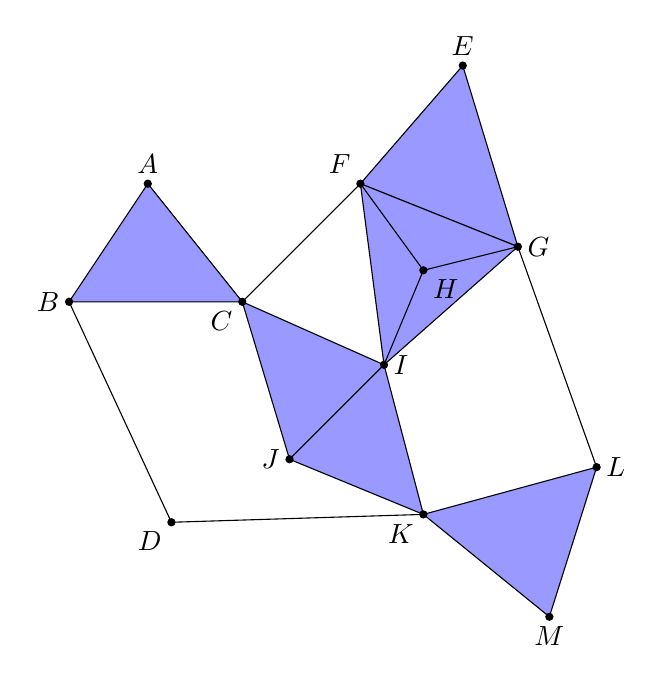
\begin{tikzpicture}[x=1cm,y=1cm]
\coordinate(A)at(1,1.5);\coordinate(B)at(0,0);\coordinate(C)at(2.2,0);\coordinate(D)at(1.3,-2.8);\coordinate(E)at(5,3);\coordinate(F)at(3.7,1.5);\coordinate(G)at(5.7,.7);\coordinate(H)at(4.5,.4);\coordinate(I)at(4,-.8);\coordinate(J)at(2.8,-2);\coordinate(K)at(4.5,-2.7);\coordinate(L)at(6.7,-2.1);\coordinate(M)at(6.1,-4);
\filldraw[fill=blue!40](A)--(B)--(C)--cycle;\filldraw[fill=blue!40](C)--(I)--(J)--cycle;\filldraw[fill=blue!40](E)--(F)--(G)--cycle;
\filldraw[fill=blue!40](F)--(G)--(I)--cycle;\draw(F)--(H)--(G);\draw(H)--(I);
\filldraw[fill=blue!40](I)--(J)--(K)--cycle;\filldraw[fill=blue!40](K)--(L)--(M)--cycle;
\draw(B)--(D)--(K);\draw(C)--(F);\draw(G)--(L);
\foreach\v/\pos in{A/above,B/left,C/below left,D/below left,E/above,F/above left,G/right,H/below right,I/right,J/left,K/below left,L/right,M/below}{\fill(\v)circle(1.5pt);\node[\pos]at(\v){$\v$};}
\end{tikzpicture}\end{center}
Trong trường hợp này, $X_1$ chứa những phần tử như $\{A,B\}$, $\{D,K\}$, nhưng không chứa $\{D,J\}$. Hãy viết $X_2,X_3,X_4$. Gợi ý: hình vẽ $X$ được chủ ý vẽ để cho biết $X_3$ có một phần tử.

\noindent\textbf{Lời giải 3.4.4.6.} $X_2$ là tập hợp các tam giác, $X_3$ là tập hợp các tứ diện, $X_4$ là tập hợp các 4-đơn hình:
\begin{align*}
X_2=\{&\{A,B,C\},\{C,I,J\},\{E,F,G\},\{F,G,H\},\{F,G,I\},\\
&\{F,H,I\},\{G,H,I\},\{I,J,K\},\{K,L,M\}\};\\
X_3&=\{\{F,G,H,I\}\};\\ X_4&=\varnothing.
\end{align*}

% Source: printed p. 100; PDF p. 109
\noindent\textbf{Bài tập 3.4.4.7.} 2-đơn hình $\Delta^2$ được vẽ thành một tam giác tô kín với các đỉnh $V=\{1,2,3\}$. Có một phức đơn hình, thường được ký hiệu $\partial\Delta^2$, được vẽ thành một tam giác rỗng có cùng tập hợp đỉnh.
\begin{enumerate}[label=\alph*.]
\item Vẽ $\Delta^2$, $\partial\Delta^2$ cạnh nhau, và thể hiện rõ sự khác biệt.
\item Viết $X=\partial\Delta^2$ như một phức đơn hình. Nói cách khác, các phần tử của các tập hợp $X_0,X_1,X_2,X_3,\ldots$ là gì?
\end{enumerate}
\noindent\textbf{Lời giải 3.4.4.7.}\keepwithnext
\begin{enumerate}[label=\alph*.]
\item
\begin{center}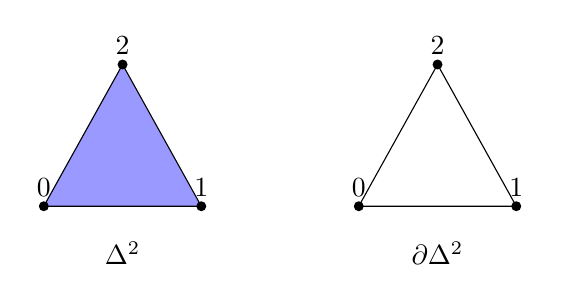
\begin{tikzpicture}
\filldraw[fill=blue!40](0,0)--(2,0)--(1,1.8)--cycle;\draw(4,0)--(6,0)--(5,1.8)--cycle;
\foreach\x/\y/\v in{0/0/0,2/0/1,1/1.8/2,4/0/0,6/0/1,5/1.8/2}{\fill(\x,\y)circle(1.8pt);\node[above]at(\x,\y){$\v$};}\node at(1,-.6){$\Delta^2$};\node at(5,-.6){$\partial\Delta^2$};
\end{tikzpicture}\end{center}
\item Có ba 0-đơn hình, $X_0=\{1,2,3\}$\ctIIInote{Bản gốc ghi $X_0=\{1,2,3\}$ nhưng hình vẽ và các cạnh của $X_1$ dùng các đỉnh $0,1,2$. Bản dịch giữ nguyên sự không khớp này vì có nhiều cách đổi nhãn.}, và ba 1-đơn hình,
\[X_1=\{\{0,1\},\{1,2\},\{0,2\}\}.\]
 Không có đơn hình chiều từ 2 trở lên, nên với $n\ge2$, ta có $X_n=\varnothing$.
\end{enumerate}

\subsubsection*{3.4.4.8\quad Bộ phân loại đối tượng con}
Cho một tập con $A\subseteq X$, ta có thể quyết định với mỗi phần tử của $X$ rằng nó có thuộc $A$ hay không. Đây là một câu hỏi đúng/sai dành cho $X$.

\noindent\textbf{Định nghĩa 3.4.4.9.} Ta định nghĩa \emph{bộ phân loại đối tượng con} (subobject classifier) của $\mathbf{Set}$, ký hiệu $\Omega$, là tập hợp $\Omega:=\{\mathrm{True},\mathrm{False}\}$ cùng hàm $\{\ctIIIface\}\to\Omega$ gửi phần tử duy nhất đến $\mathrm{True}$.

% Source: printed p. 101; PDF p. 110
\noindent\textbf{Mệnh đề 3.4.4.10.} \emph{Cho $X$ là một tập hợp. Có một đẳng cấu}
\[\phi:\operatorname{Hom}_{\mathbf{Set}}(X,\Omega)\xrightarrow{\cong}\mathbb P(X).\]
\begin{proof}[Chứng minh]
Cho một hàm $f:X\to\Omega$, đặt $\phi(f)=\{x\in X\mid f(x)=\mathrm{True}\}\subseteq X$. Bây giờ, ta xây dựng một hàm $\psi:\mathbb P(X)\to\operatorname{Hom}_{\mathbf{Set}}(X,\Omega)$ làm nghịch đảo của $\phi$. Cho một tập con $A\subseteq X$, ta định nghĩa\ctIIInote{Bản gốc in $\psi(i)(x)$; ở đây dùng $\psi(A)(x)$ vì $A$ là tập con được cho.}
\begin{equation*}\psi(A):X\to\Omega\quad\text{bởi }\psi(A)(x)=\begin{cases}\mathrm{True}&\text{nếu }x\in A,\\\mathrm{False}&\text{nếu }x\notin A.\end{cases}\tag{3.25}\end{equation*}
Dễ dàng kiểm tra rằng $\phi,\psi$ là nghịch đảo của nhau.
\end{proof}

\noindent\textbf{Khẩu quyết 3.4.4.11.}\keepwithnext
\begin{quote}Một hàm từ $X$ đến $\Omega=\{\mathrm{True},\mathrm{False}\}$ giống như việc điểm danh. Ta quan tâm đến tập con gọi lên ``$\mathrm{True}$''.\end{quote}

\noindent\textbf{Định nghĩa 3.4.4.12 (Hàm đặc trưng).} Cho một tập con $A\subseteq X$. Ta định nghĩa \emph{hàm đặc trưng của $A$ trong $X$} là hàm $\psi(A):X\to\Omega$ trong (3.25).

Cho $X$ là một tập hợp bất kỳ và $\mathbb P(X)$ là tập lũy thừa của nó. Theo Mệnh đề 3.4.4.10, có một song ánh giữa $\mathbb P(X)$ và $\Omega^X$. Vì $\Omega$ có hai phần tử, số phần tử của $\mathbb P(X)$ là $2^{|X|}$, giải thích câu trả lời đúng của Bài tập 3.4.4.2.

\noindent\textbf{Bài tập 3.4.4.13.} Cho $f:X\to\Omega$ là hàm đặc trưng của một tập con $A\subseteq X$, và định nghĩa phần bù của nó là $A'=X-A$, tức $A'=\{x\in X\mid x\notin A\}$.
\begin{enumerate}[label=\alph*.]
\item Hàm đặc trưng của $A'\subseteq X$ là gì?
\item Bạn có thể biểu diễn nó bằng $f$ và một hàm $\Omega\to\Omega$ nào đó không?
\end{enumerate}
\noindent\textbf{Lời giải 3.4.4.13.} Ta giải cả hai phần cùng lúc. Gọi $c:\Omega\to\Omega$ là hàm gửi $\mathrm{True}$ đến $\mathrm{False}$ và gửi $\mathrm{False}$ đến $\mathrm{True}$. Khi đó, hàm đặc trưng của $A'\subseteq X$ là hợp thành
\[X\xrightarrow{f}\Omega\xrightarrow{c}\Omega.\]

% Source: printed p. 102; PDF p. 111
\subsection{Toàn ánh, đơn ánh}
Định nghĩa cổ điển của đơn ánh và toàn ánh trong Định nghĩa 3.4.5.1 sử dụng phần tử. Nhưng một khái niệm vững chắc hơn sử dụng hàm; nó được cho trong Mệnh đề 3.4.5.8.

\noindent\textbf{Định nghĩa 3.4.5.1.} Cho $f:X\to Y$ là một hàm.
\begin{itemize}
\item Ta nói $f$ là \emph{đơn ánh} nếu với mọi $x,x'\in X$ thỏa mãn $f(x)=f(x')$, ta có $x=x'$.
\item Ta nói $f$ là \emph{toàn ánh} nếu với mọi $y\in Y$, tồn tại $x\in X$ sao cho $f(x)=y$.
\item Ta nói $f$ là \emph{song ánh} nếu nó vừa đơn ánh vừa toàn ánh.
\end{itemize}
Đôi khi ta ký hiệu một hàm đơn ánh là $X\hookrightarrow Y$, một hàm toàn ánh là $X\twoheadrightarrow Y$, một hàm song ánh là $X\xrightarrow{\cong}Y$ (xem Mệnh đề 3.4.5.4).

\noindent\textbf{Bài tập 3.4.5.2.}\keepwithnext
\begin{enumerate}[label=\alph*.]
\item Hàm $f:\mathbb Z\to\mathbb N$, $f(n)=n^2$, là đơn ánh, toàn ánh hay không thuộc loại nào?
\item Hàm $g:\mathbb N\to\mathbb N$, $g(n)=n^2$, là đơn ánh, toàn ánh hay không thuộc loại nào?
\item Hàm $h:\mathbb Z\to\mathbb N$, $h(n)=|n|$ (giá trị tuyệt đối), là đơn ánh, toàn ánh hay không thuộc loại nào?
\item Hàm $i:\mathbb Z\to\mathbb Z$, $i(n)=-n$, là đơn ánh, toàn ánh hay không thuộc loại nào?
\end{enumerate}
\noindent\textbf{Lời giải 3.4.5.2.}\keepwithnext
\begin{enumerate}[label=\alph*.]
\item Không thuộc loại nào. Vì $f(-1)=f(1)$, nó không thể đơn ánh. Vì không số nguyên $n\in\mathbb Z$ nào thỏa mãn $f(n)=2$\ctIIInote{Bản gốc in $f(n)\ne2$. Ở đây sửa thành $f(n)=2$: không có số nguyên nào có bình phương bằng $2$, nên $f$ không toàn ánh.}, nó không thể toàn ánh.
\item Nó đơn ánh nhưng không toàn ánh.
\item Nó toàn ánh nhưng không đơn ánh.
\item Nó song ánh, tức vừa đơn ánh vừa toàn ánh.
\end{enumerate}

\noindent\textbf{Bài tập 3.4.5.3.} Cho $f:X\to Y$, $g:Y\to Z$ là các hàm.
% Source: printed p. 103; PDF p. 112
\begin{enumerate}[label=\alph*.]
\item Chứng minh rằng nếu $f,g$ là các đơn ánh thì $g\circ f$ cũng là đơn ánh.
\item Chứng minh rằng nếu $f,g$ đều là toàn ánh thì $g\circ f$ cũng là toàn ánh.
\item Chứng minh rằng nếu $g\circ f$ là đơn ánh thì $f$ cũng là đơn ánh.
\item Chứng minh rằng nếu $g\circ f$ là toàn ánh thì $g$ cũng là toàn ánh.
\end{enumerate}
\noindent\textbf{Lời giải 3.4.5.3.}\keepwithnext
\begin{enumerate}[label=\alph*.]
\item Cho $x,x'\in X$ và giả sử $(g\circ f)(x)=(g\circ f)(x')$. Khi đó $g(f(x))=g(f(x'))$, nên tính đơn ánh của $g$ suy ra $f(x)=f(x')$; tính đơn ánh của $f$ suy ra $x=x'$.
\item Cho $z\in Z$. Tính toàn ánh của $g$ suy ra tồn tại $y\in Y$ sao cho $g(y)=z$; tính toàn ánh của $f$ suy ra tồn tại $x\in X$ sao cho $f(x)=y$.
\item Cho $x,x'\in X$ và giả sử $f(x)=f(x')$. Vì $g$ là một hàm, $(g\circ f)(x)=(g\circ f)(x')$; lúc này, tính đơn ánh của $g\circ f$ suy ra $x=x'$.
\item Cho $z\in Z$. Tính toàn ánh của $g\circ f$ suy ra tồn tại $x\in X$ sao cho $(g\circ f)(x)=z$. Nhưng như vậy ta đã tìm được $y:=f(x)\in Y$ sao cho $g(y)=z$.
\end{enumerate}

\noindent\textbf{Mệnh đề 3.4.5.4.} \emph{Một hàm $f:X\to Y$ là song ánh khi và chỉ khi nó là một đẳng cấu.}
\begin{proof}[Chứng minh]
Giả sử $f$ song ánh; ta định nghĩa một nghịch đảo $g:Y\to X$. Với mỗi $y\in Y$, nghịch ảnh $f^{-1}(y)\subseteq X$ là một tập hợp có đúng một phần tử. Thật vậy, nó có ít nhất một phần tử vì $f$ toàn ánh và nhiều nhất một phần tử vì $f$ đơn ánh. Định nghĩa $g(y)$ là phần tử duy nhất của $f^{-1}(y)$. Dễ thấy $f,g$ là nghịch đảo của nhau.

Chú ý rằng với mỗi tập hợp $X$, hàm đồng nhất $\mathrm{id}_X:X\to X$ là song ánh. Bây giờ, giả sử $f$ là một đẳng cấu và $g$ là nghịch đảo của nó. Hợp thành $g\circ f=\mathrm{id}_X$ là đơn ánh và hợp thành $f\circ g=\mathrm{id}_Y$ là toàn ánh, nên $f$ đơn ánh và toàn ánh theo Bài tập 3.4.5.3.
\end{proof}

\noindent\textbf{Mệnh đề 3.4.5.5.} \emph{Cho $m,n\in\mathbb N$ là các số tự nhiên. Khi đó $m\le n$ khi và chỉ khi tồn tại một đơn ánh $\underline m\hookrightarrow\underline n$.}
\begin{proof}[Phác thảo chứng minh]
Nếu $m\le n$, có một phép bao hàm
\[\{1,2,\ldots,m\}\to\{1,2,\ldots,n\}.\]
Bây giờ, giả sử ta được cho một đơn ánh $f:\underline m\to\underline n$; ta giả sử $m>n$ rồi suy ra một
% Source: printed p. 104; PDF p. 113
mâu thuẫn. Nếu $m>n$ thì $n+1\le m$, và ta đã chỉ ra rằng tồn tại một đơn ánh
\[g:\underline{n+1}\hookrightarrow\underline m.\]
Lấy hợp thành, ta có một đơn ánh\ctIIInote{Bản gốc in $h:=g\circ f$. Theo các miền và đối miền đã cho, hợp thành từ $\underline{n+1}$ đến $\underline n$ là $f\circ g$.}
\[h:=f\circ g:\underline{n+1}\hookrightarrow\underline n.\]
Theo Bài tập 3.4.5.3, hợp thành này là đơn ánh. Có thể dùng quy nạp theo $n$ để chứng minh điều này không thể xảy ra.
\end{proof}

\noindent\textbf{Hệ quả 3.4.5.6.} \emph{Cho $m,n\in\mathbb N$ là các số tự nhiên. Khi đó $m=n$ khi và chỉ khi tồn tại một đẳng cấu $f:\underline m\xrightarrow{\cong}\underline n$.}
\begin{proof}[Chứng minh]
Nếu $m=n$, hàm đồng nhất $\mathrm{id}_{\underline m}:\underline m\to\underline n$ là một đẳng cấu.

Ngược lại, nếu ta có một đẳng cấu $f:\underline m\xrightarrow{\cong}\underline n$, thì cả nó và nghịch đảo của nó đều là đơn ánh theo Mệnh đề 3.4.5.4. Vì thế, $m\le n$ và $n\le m$ theo Mệnh đề 3.4.5.5, suy ra $m=n$.
\end{proof}

\noindent\textbf{Định nghĩa 3.4.5.7 (Đơn cấu, toàn cấu).} Cho $f:X\to Y$ là một hàm. Ta nói $f$ là một \emph{đơn cấu} (monomorphism) nếu với mọi tập hợp $A$ và mọi cặp hàm $g,g':A\to X$,
% Source diagram: Art_P79.jpg
\[\begin{tikzcd}A\arrow[r,bend left=15,"g"]\arrow[r,bend right=15,"g'"']&X\arrow[r,"f"]&Y\end{tikzcd}\]
nếu $f\circ g=f\circ g'$ thì $g=g'$.

Ta nói $f$ là một \emph{toàn cấu} (epimorphism) nếu với mọi tập hợp $B$ và mọi cặp hàm $h,h':Y\to B$,
% Source diagram: Art_P80.jpg
\[\begin{tikzcd}X\arrow[r,"f"]&Y\arrow[r,bend left=15,"h"]\arrow[r,bend right=15,"h'"']&B\end{tikzcd}\]
nếu $h\circ f=h'\circ f$ thì $h=h'$.

\noindent\textbf{Mệnh đề 3.4.5.8.} \emph{Cho $f:X\to Y$ là một hàm. Khi đó $f$ đơn ánh khi và chỉ khi nó là đơn cấu; $f$ toàn ánh khi và chỉ khi nó là toàn cấu.}
\begin{proof}[Chứng minh]
Ta dùng ký hiệu như trong Định nghĩa 3.4.5.7.

Nếu $f$ là đơn cấu, rõ ràng nó đơn ánh khi đặt $A=\{\ctIIIface\}$. Giả sử $f$ đơn ánh và cho các hàm $g,g':A\to X$ sao cho $f\circ g=f\circ g'$, nhưng để tìm mâu thuẫn, giả sử $g\ne g'$. Khi đó tồn tại $a\in A$ sao cho $g(a)\ne g'(a)\in X$. Nhưng tính đơn ánh suy ra $f(g(a))\ne f(g'(a))$, mâu thuẫn với $f\circ g=f\circ g'$.

Giả sử $f:X\to Y$ là toàn cấu, và chọn một $y_0\in Y$ (chú ý rằng nếu $Y$ rỗng thì khẳng định đúng một cách hiển nhiên). Đặt $B=\Omega$, cho $h:Y\to\Omega$ là
% Source: printed p. 105; PDF p. 114
hàm đặc trưng của tập con $\{y_0\}\subseteq Y$ và $h':Y\to\Omega$ là hàm đặc trưng của $\varnothing\subseteq Y$. Chú ý rằng $h(y)=h'(y)$ với mọi $y\ne y_0$. Vì $f$ là toàn cấu và $h\ne h'$, ta phải có $h\circ f\ne h'\circ f$, nên tồn tại $x\in X$ với $h(f(x))\ne h'(f(x))$; điều này suy ra $f(x)=y_0$. Vậy $f$ toàn ánh.

Cuối cùng, giả sử $f$ toàn ánh và cho các hàm $h,h':Y\to B$ với $h\circ f=h'\circ f$. Với mọi $y\in Y$, tồn tại $x\in X$ sao cho $f(x)=y$, nên $h(y)=h(f(x))=h'(f(x))=h'(y)$. Điều đó chứng minh $f$ là toàn cấu.
\end{proof}

\noindent\textbf{Mệnh đề 3.4.5.9.} \emph{Cho $g:A\to Y$ là một đơn cấu. Với mọi hàm $f:X\to Y$, ánh xạ bên trái $g':X\times_YA\to X$ trong biểu đồ}
% Source diagram: Art_P81.jpg
\[\begin{tikzcd}X\times_YA\arrow[r,"f'"]\arrow[d,"g'"']\arrow[dr,phantom,"\lrcorner",very near start]&A\arrow[d,"g"]\\X\arrow[r,"f"']&Y\end{tikzcd}\]
\emph{là một đơn cấu.}
\begin{proof}[Chứng minh]
Để chứng minh $g'$ là đơn cấu, ta lấy một tập hợp tùy ý $B$ và hai ánh xạ $m,n:B\to X\times_YA$ sao cho $g'\circ m=g'\circ n$, và ký hiệu hàm ấy là $p:=g'\circ m:B\to X$. Đặt $q=f'\circ m$, $r=f'\circ n$. Biểu đồ có dạng:
% Source diagram: Art_P82.jpg
\[\begin{tikzcd}[column sep=large,row sep=large]
B\arrow[d,bend right=8,"m"']\arrow[d,bend left=8,"n"]\arrow[dd,bend right=55,"p"']\arrow[dr,bend left=15,"q"]\arrow[dr,bend right=15,"r"']&\\
X\times_YA\arrow[r,"f'"']\arrow[d,"g'"']&A\arrow[d,"g"]\\X\arrow[r,"f"']&Y
\end{tikzcd}\]
Ta có
\begin{align*}
g\circ q&=g\circ f'\circ m=f\circ g'\circ m=f\circ p\\
&=f\circ g'\circ n=g\circ f'\circ n=g\circ r.
\end{align*}
Nhưng đã giả sử $g$ là đơn cấu, nên điều này suy ra $q=r$. Theo tính chất phổ dụng của kéo lui, Mệnh đề 3.2.1.15, ta có $m=n=\langle p,q\rangle_Y:B\to X\times_YA$.\ctIIInote{Bản gốc in $\langle q,p\rangle_Y$. Với thứ tự các thừa số $X\times_YA$ đã cho, thành phần đầu là $p:B\to X$, thành phần sau là $q:B\to A$; vì vậy dùng $\langle p,q\rangle_Y$.}
\end{proof}

% Source: printed p. 106; PDF p. 115
\noindent\textbf{Ví dụ 3.4.5.10.} Giả sử một olog có hình vuông tích thớ
% Source diagram: Art_P83.jpg
\[\begin{tikzcd}X\times_YA\arrow[r,"f'"]\arrow[d,"g'"']\arrow[dr,phantom,"\lrcorner",very near start]&A\arrow[d,"g"]\\X\arrow[r,"f"']&Y\end{tikzcd}\]
trong đó $g$ được dự định là một đơn cấu và $f$ là một ánh xạ bất kỳ.\footnote{Dĩ nhiên, biểu đồ này đối xứng, nên các ý tưởng tương tự vẫn đúng nếu $f$ là một đơn cấu còn $g$ là một ánh xạ bất kỳ.} Khi đó, có các hệ thống gắn nhãn cho $f',g'$ và $X\times_YA$. Cụ thể,
\begin{itemize}
\item ``là'' là một nhãn phù hợp cho $g,g'$;
\item nhãn của $f$ là một nhãn phù hợp cho $f'$;
\item $\langle\!\langle X\times_YA\rangle\!\rangle:=$ ``$\langle\!\langle X\rangle\!\rangle$ mà $\langle\!\langle f\rangle\!\rangle$ $\langle\!\langle A\rangle\!\rangle$'' là một nhãn phù hợp cho $X\times_YA$.
\end{itemize}
Một ví dụ tường minh:
% Source diagram: Art_P84.jpg
\[\begin{tikzcd}[column sep=2cm,row sep=large]
|[draw,inner sep=4pt]|\begin{gathered}X\times_YA\\\text{một xương sườn được}\\\text{tạo ra bởi một con bò}\end{gathered}\arrow[r,"\substack{\text{được tạo ra}\\\text{bởi}}"]\arrow[d,"\text{là}"']\arrow[dr,phantom,"\lrcorner",very near start]&|[draw,inner sep=4pt]|\begin{gathered}A\\\text{một con bò}\end{gathered}\arrow[d,"\text{là}"]\\
|[draw,inner sep=4pt]|\begin{gathered}X\\\text{một xương sườn}\end{gathered}\arrow[r,"\substack{\text{được tạo ra}\\\text{bởi}}"']&|[draw,inner sep=4pt]|\begin{gathered}Y\\\text{một động vật}\end{gathered}
\end{tikzcd}\]

\noindent\textbf{Hệ quả 3.4.5.11.} \emph{Cho $i:A\to X$ là một đơn cấu và $\mathrm{True}:\{\ctIIIface\}\to\Omega$ là bộ phân loại đối tượng con (xem Định nghĩa 3.4.4.9). Khi đó, có một hình vuông tích thớ dạng}
% Source diagram: Art_P85.jpg
\begin{equation*}\begin{tikzcd}A\arrow[r,"f'"]\arrow[d,"i"']\arrow[dr,phantom,"\lrcorner",very near start]&\{\ctIIIface\}\arrow[d,"\mathrm{True}"]\\X\arrow[r,"f"']&\Omega\end{tikzcd}\tag{3.26}\end{equation*}
\begin{proof}[Chứng minh]
Cho $X'\subseteq X$ là ảnh của $i$, và $f:X\to\Omega$ là hàm đặc trưng của $X'\subseteq X$, được cho bởi Mệnh đề 3.4.4.10. Khi đó, dễ dàng kiểm tra rằng biểu đồ (3.26) là một kéo lui.
\end{proof}
